%% LyX 2.3.6.1 created this file.  For more info, see http://www.lyx.org/.
%% Do not edit unless you really know what you are doing.
\documentclass[english]{article}
\usepackage[T1]{fontenc}
\usepackage[latin9]{inputenc}
\usepackage{amsmath}
\usepackage{graphicx}
\usepackage{babel}
\begin{document}
The smooth curve in baryon loop diagram like 
\begin{figure}
\includegraphics[scale=0.5]{pic/gpdH-b-noD}

\includegraphics[scale=0.5]{pic/gpdE-b-noD}

\caption{H and E from diagram b}

\end{figure}

exists because in baryon loop we do not include the D term in convolution
calculation like the meson loop.

The convolution formula for baryon loop 
\begin{align*}
\int_{x}^{1}d(1-y)\frac{1}{1-y}f(y,\xi,t)H_{q}(\frac{x}{1-y},\frac{\xi}{1-y},t),\quad1-y & >x>\xi\\
\int_{\xi}^{1}d(1-y)\frac{1}{1-y}f(y,\xi,t)H_{q}(\frac{x}{1-y},\frac{\xi}{1-y},t),\quad1-y & >\xi>x\\
\int_{-\xi}^{\xi}d(1-y)\frac{1}{2\xi}f(y,\xi,t)\frac{1}{\pi}\frac{\xi}{1-y}\int_{s_{0}}^{\infty}ds\frac{Im\Phi(\frac{\frac{x}{\xi}+1}{2},\frac{\frac{1-y}{\xi}+1}{2},s)}{s-t+i\epsilon}\quad\xi & >\{1-y,|x|\}\\
\int_{-x}^{1}d(1-y)\frac{1}{1-y}f(y,\xi,t)H_{q}(\frac{x}{1-y},\frac{\xi}{1-y},t),\quad- & \xi>x>-1
\end{align*}

and for meson loop
\begin{align*}
\int_{x}^{1}dy\frac{1}{y}f(y,\xi,t)H_{q}(\frac{x}{y},\frac{\xi}{y},t),\quad y & >x>\xi\\
\int_{\xi}^{1}dy\frac{1}{y}f(y,\xi,t)H_{q}(\frac{x}{y},\frac{\xi}{y},t),\quad y & >\xi>x\\
\int_{-\xi}^{\xi}dy\frac{1}{2\xi}f(y,\xi,t)\frac{\xi}{\pi y}\int_{s_{0}}^{\infty}ds\frac{Im\Phi(\frac{\frac{x}{\xi}+1}{2},\frac{\frac{y}{\xi}+1}{2},s)}{s-t+i\epsilon}\quad\xi & >\{y,|x|\}\\
\int_{-x}^{1}dy\frac{1}{y}f(y,\xi,t)H_{q}(\frac{x}{y},\frac{\xi}{y},t),\quad- & \xi>x>-1
\end{align*}

The input GPD $H_{q}$ and GDA $\Phi$ are both in so called double
distribution representation and they have this form 
\begin{align*}
H(x,\xi,t) & =\int_{-1}^{1}d\beta\int_{-1+|\beta|}^{1-|\beta|}d\alpha\delta(x-\beta-\alpha\xi)h(\beta,\alpha,t)\\
E(x,\xi,t) & =\int_{-1}^{1}d\beta\int_{-1+|\beta|}^{1-|\beta|}d\alpha\delta(x-\beta-\alpha\xi)e(\beta,\alpha,t)\\
\Phi_{1}(z,\eta,s) & =2(2\eta-1)\int_{-1}^{1}d\beta\int_{-1+|\beta|}^{1-|\beta|}d\alpha\delta(2z-1-(2\eta-1)\beta-\alpha)h_{0}(\beta,\alpha)H(\beta,0,s)
\end{align*}

In double distribution representation, the first moment of GPD do
not have D term which is observed by experiment, and a easy way to
solve this is add a extra term in formula above which is
\begin{align*}
H(x,\xi,t) & =\int_{-1}^{1}d\beta\int_{-1+|\beta|}^{1-|\beta|}d\alpha\delta(x-\beta-\alpha\xi)h(\beta,\alpha,t)+D(\frac{x}{\xi},t)\theta(\xi-|x|)\\
\Phi_{1}(z,\eta,s) & =2(2\eta-1)\int_{-1}^{1}d\beta\int_{-1+|\beta|}^{1-|\beta|}d\alpha\delta(2z-1-(2\eta-1)\beta-\alpha)h_{0}(\beta,\alpha)H(\beta,0,s)\\
 & +D(1-2z,t)\theta(1-|1-2z|)
\end{align*}

The problem is in GDA case
\[
\int_{-\xi}^{\xi}d(1-y)\frac{1}{2\xi}f(y,\xi,t)\frac{1}{\pi}\frac{\xi}{1-y}\int_{s_{0}}^{\infty}ds\frac{Im\Phi(\frac{\frac{x}{\xi}+1}{2},\frac{\frac{1-y}{\xi}+1}{2},s)}{s-t+i\epsilon}
\]

when we consider the D-term part 
\begin{gather*}
\int_{-\xi}^{\xi}d(1-y)\frac{1}{2}f(y,\xi,t)\frac{1}{1-y}D(\frac{x}{\xi},t)\\
\int_{-\xi}^{\xi}dy\frac{1}{2}f(y,\xi,t)\frac{1}{y}D(\frac{x}{\xi},t)
\end{gather*}

Obviously we have a pole in $y=0\textrm{and}\bar{y}=1-y=0$. In meson
case, $\int_{-\xi}^{\xi}dy\frac{1}{2}f(y,\xi,t)\frac{1}{y}D(\frac{x}{\xi},t)$,
the splitting function is always 0 at $y=0$ which cancel the pole.
In baryon loop case, we can not cancel the divergence.

In early calculation, I do not consider the D-term in baryon loop,
and this will make the result of GPD has a smooth curve. It can be
checked by the result of diagram a. The different lines in Fig.2 and
Fig.3 represent the different input in convolution calculation. For
orange line, the input is GPD, for black line, the input is GDA and
the blue line is the combine of GPD and GDA. The red line is result
with GPD input in DGLAP region. 

\begin{figure}
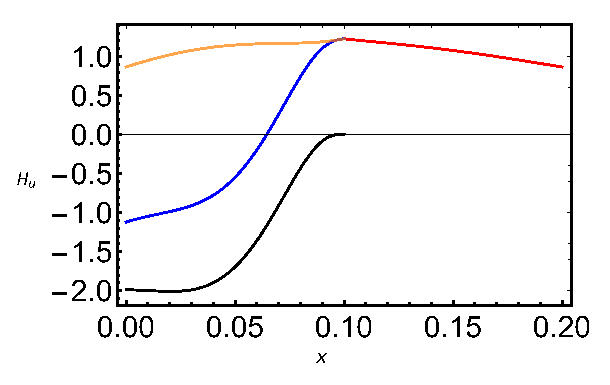
\includegraphics{pic/h-a-2d-D}\caption{original result of $H_{u}(x,\xi,t)$ from diagram a, where $\xi=0.1\ t=-1$}

\end{figure}

\begin{figure}
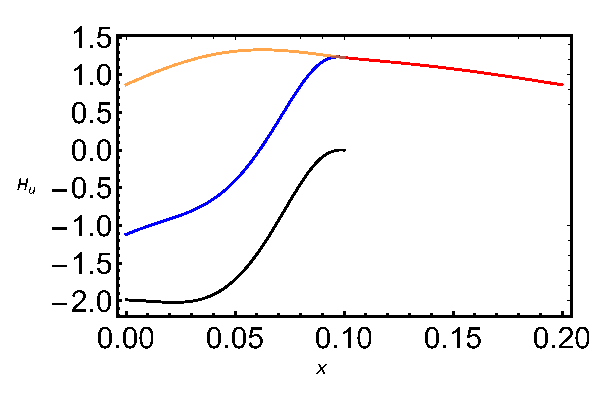
\includegraphics{pic/h-a-2d-noD}

\caption{same result as Fig.2 only without D term in ERBL region}

\end{figure}

The D-term in baryon loop may act like $\int_{-\xi}^{\xi}dy\frac{1}{y}=0$,
where the divergence around $1-y=0$ cancel with each other and we
can get a converged result. The integral which contain divergence
is 
\[
\int_{-\xi}^{\xi}d(1-y)f(y,\xi,t)\frac{1}{1-y}D(\frac{x}{\xi},t)
\]

The function 
\[
F(y,x,\xi,t)=f(y,\xi,t)\frac{1}{1-y}D(\frac{x}{\xi},t)
\]

gives a curve like where we chose $D(x,t)=\frac{15x(1-x^{2})D(t)}{4},\ D(t)=\frac{\alpha}{(1-\frac{t}{\Lambda^{2}})^{2}}$
from lattice result.
\begin{figure}
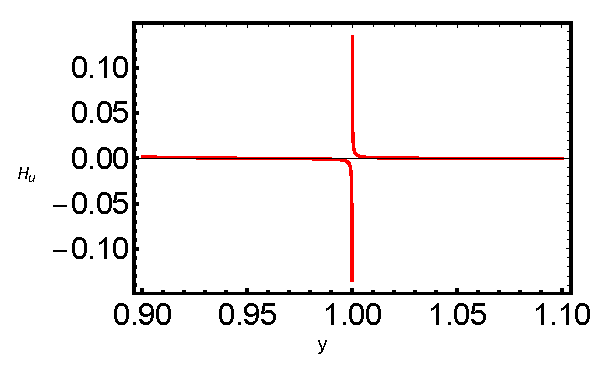
\includegraphics{pic/hd-b-2d}\caption{$F(y,-0.01,0.1,-1)$from diagram b}

\end{figure}

Change the integral in this way
\begin{gather*}
\int_{-\xi}^{\xi}d(1-y)f(y,\xi,t)\frac{1}{1-y}D(\frac{x}{\xi},t)\\
=\int_{1-\xi}^{1+\xi}d(y)f(y,\xi,t)\frac{1}{1-y}D(\frac{x}{\xi},t)\\
=\int_{1-\xi}^{1-a}d(y)f(y,\xi,t)\frac{1}{1-y}D(\frac{x}{\xi},t)+\int_{1-a}^{1+a}d(y)f(y,\xi,t)\frac{1}{1-y}D(\frac{x}{\xi},t)+\int_{1+a}^{1+\xi}d(y)f(y,\xi,t)\frac{1}{1-y}D(\frac{x}{\xi},t)
\end{gather*}

We only calculate the first and second integral to avoid the pole
\begin{gather*}
\underset{a\rightarrow0}{\textrm{Lim}}\int_{1-\xi}^{1-a}d(y)f(y,\xi,t)\frac{1}{1-y}D(\frac{x}{\xi},t)+\int_{1+a}^{1+\xi}d(y)f(y,\xi,t)\frac{1}{1-y}D(\frac{x}{\xi},t)\\
=\int_{1-\xi}^{1+\xi}d(y)f(y,\xi,t)\frac{1}{1-y}D(\frac{x}{\xi},t)
\end{gather*}

And if the divergence around $1-y=0$ cancel we have $\int_{1-a}^{1+a}d(y)f(y,\xi,t)\frac{1}{1-y}D(\frac{x}{\xi},t)=0$
when $a$ is small enough which is equal to the integral above is
same with different $a$.
\[
I(a)=\int_{1-\xi}^{1-a}d(y)f(y,\xi,t)\frac{1}{1-y}D(\frac{x}{\xi},t)+\int_{1+a}^{1+\xi}d(y)f(y,\xi,t)\frac{1}{1-y}D(\frac{x}{\xi},t)
\]

\begin{align*}
I(0.01) & =0.00002284065045\\
I(10^{-4}) & =0.00001941004441\\
I(10^{-6}) & =0.0000193752819\\
I(10^{-8}) & =0.0000193749343\\
I(10^{-10}) & =0.0000193749308
\end{align*}

This integral $\int_{1-\xi}^{1-a}d(y)f(y,\xi,t)\frac{1}{1-y}D(\frac{x}{\xi},t)$
is relatively small compared to the normal $\frac{1}{x}$ integral,
like $\int_{-0.1}^{-a}dx\frac{1}{x}$. For example 
\[
I_{1}(a)=\int_{1-\xi}^{1-a}d(y)f(y,\xi,t)\frac{1}{1-y}D(\frac{x}{\xi},t)
\]
\begin{align*}
I_{1}(0.01) & =0.00001580367639\\
I_{1}(10^{-4}) & =-0.00002524554336\\
I_{1}(10^{-6}) & =-0.00006466894493\\
I_{1}(10^{-8}) & =-0.0001040750182\\
I_{1}(10^{-10}) & =-0.0001434809205
\end{align*}

and the $\int_{-0.1}^{-a}dx\frac{1}{x}$ is 
\begin{align*}
\int_{-0.1}^{-a}dx\frac{1}{x}|_{a=0.01} & =-2.30259\\
\int_{-0.1}^{-a}dx\frac{1}{x}|_{a=10^{-4}} & =-6.90776\\
\int_{-0.1}^{-a}dx\frac{1}{x}|_{a=10^{-6}} & =-11.5129\\
\int_{-0.1}^{-a}dx\frac{1}{x}|_{a=10^{-8}} & =-16.1181\\
\int_{-0.1}^{-a}dx\frac{1}{x}|_{a=10^{-10}} & =-20.7233
\end{align*}

The reason is the numerator in $I_{1}(a)$ which is $f(y,\xi,t)D(\frac{x}{\xi},t)$
is very small, the curve of $f(y,0.1,-1)$ is while $D(\frac{-0.01}{0.1},-1)=0.0326303$

\begin{figure}
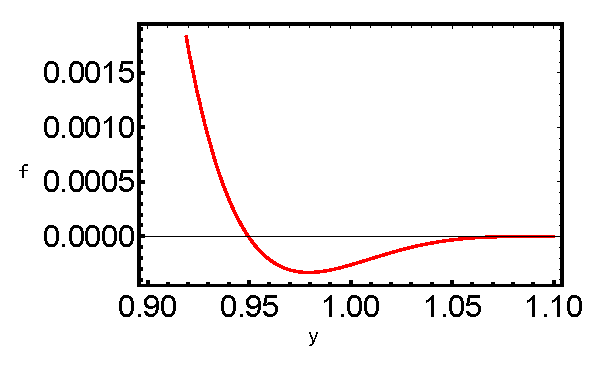
\includegraphics{pic/f-b-2d-full}

\caption{$f(y,0.1,-1)$}

\end{figure}

and this makes $I_{1}(a)$ is more like $\int_{-0.1}^{-a}dx\frac{0.00001}{x}$
. And the numerical integral in mathematica can not give a divergent
result even for $\int_{-0.1}^{-a}dx\frac{1}{x}$, which will lost
precision when $a<10^{-60}$ and for $a>10^{-60}$, the result of
$\int_{-0.1}^{-a}dx\frac{1}{x}>-135.853$

The result of GPD from diagram b if we add D-term is 
\begin{figure}
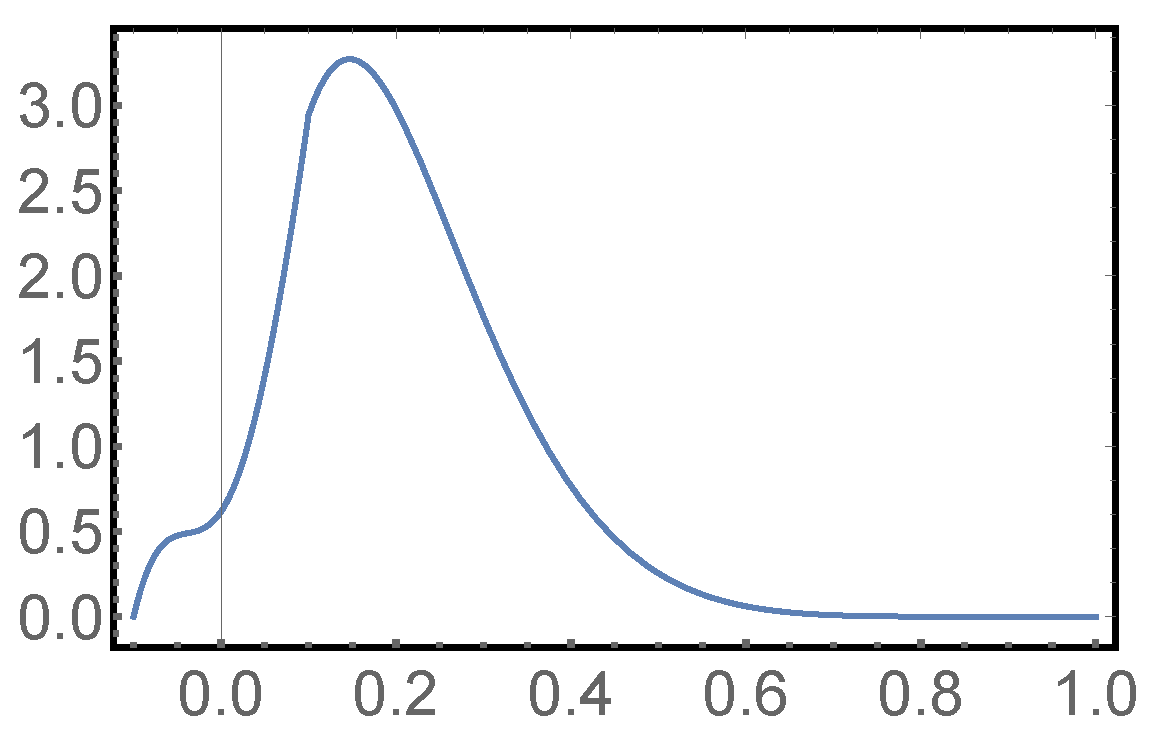
\includegraphics[scale=0.5]{pic/gpdH-b-D}

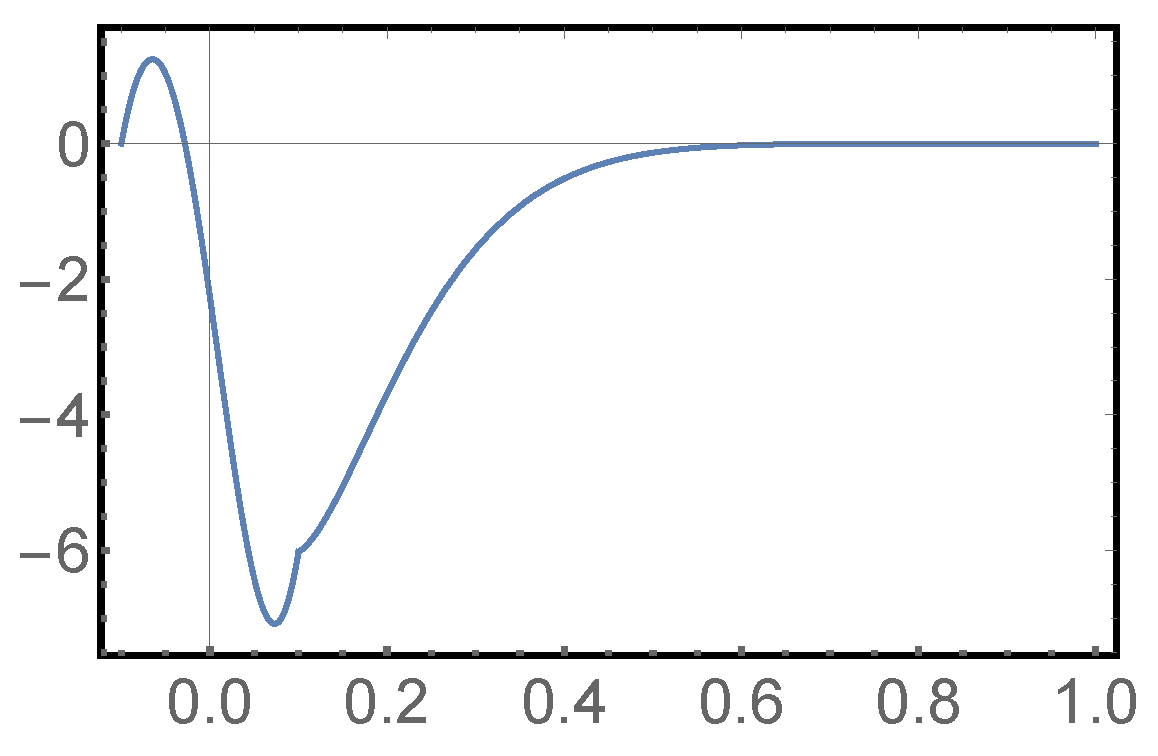
\includegraphics[scale=0.5]{pic/gpdE-b-D}

\caption{H and E from diagram b}
\end{figure}

\begin{figure}
\includegraphics[scale=0.5]{pic/gpdH-b-noD}

\includegraphics[scale=0.5]{pic/gpdE-b-noD}

\caption{H and E from diagram b}
\end{figure}

\end{document}
